\documentclass[a4paper]{article}

\usepackage[utf8]{inputenc}
\usepackage{lmodern}
\usepackage[T1]{fontenc}
\usepackage[babel=true]{microtype}
\usepackage[portuguese]{babel}
\usepackage[pdftex]{hyperref}
\usepackage{graphicx}
\usepackage{eurosym}
\usepackage{scrextend}
\usepackage{hyphenat}
\usepackage{url}
\usepackage{hyperref}
\usepackage{float}
\usepackage{indentfirst}
\usepackage{verbatim}
\usepackage{listings}
\usepackage[usenames,dvipsnames,svgnames,table]{xcolor}

\lstdefinestyle{customprolog}{
  belowcaptionskip=1\baselineskip,
  breaklines=true,
  xleftmargin=\parindent,
  language=Prolog,
  showstringspaces=false,
  tabsize=2,
  basicstyle=\footnotesize\ttfamily,
  keywordstyle=\bfseries\color{blue},
  commentstyle=\itshape\color{gray},
  identifierstyle=\color{black},
  stringstyle=\color{OliveGreen},
}

\begin{document}

\setlength{\textwidth}{16cm}
\setlength{\textheight}{22cm}

\title{\Huge\textbf{Jogo Cage}\linebreak\linebreak\linebreak
\Large\textbf{Relatório Final}\linebreak\linebreak
\linebreak\linebreak

\includegraphics[scale=0.1]{resources/feup-logo.png}\linebreak\linebreak
\linebreak\linebreak
\Large{Mestrado Integrado em Engenharia Informática e Computação} \linebreak\linebreak
\Large{Programação em Lógica}\linebreak
}

\author{\textbf{Grupo 2:}\\ José Peixoto - 200603103 \\ Luís Cruz - 201303248 \\\linebreak\linebreak \\
 \\ Faculdade de Engenharia da Universidade do Porto \\ Rua Roberto Frias, s\/n, 4200-465 Porto, Portugal \linebreak\linebreak\linebreak
\linebreak\linebreak\vspace{1cm}}
%\date{Junho de 2007}
\maketitle
\thispagestyle{empty}

%************************************************************************************************
%************************************************************************************************

\newpage

\section*{Resumo}
Resumo sucinto do trabalho com 150 a 250 palavras (problema abordado, objetivo, como foi o problema resolvido/abordado, principais resultados e conclusões).

No âmbito da unidade curricular de Programação em Lógica, foi-nos proposto o desenvolvimento de um jogo de tabuleiro em \emph{Prolog}: o \emph{Cage}. O principal objetivo na realização deste projeto foi a aquisição de novas competências na expressão de conceitos lógicos em \emph{Prolog}.

Findo o projeto, realçamos a expressividade do \emph{Prolog} para conceitos lógicos, e a nossa carência de experiência com este paradigma de programação.

\newpage

\tableofcontents

%************************************************************************************************
%************************************************************************************************

%*************************************************************************************************
%************************************************************************************************

\newpage

%%%%%%%%%%%%%%%%%%%%%%%%%%
\section{Introdução}

Descrever os objetivos e motivação do trabalho. Descrever num parágrafo breve a estrutura do relatório.


%%%%%%%%%%%%%%%%%%%%%%%%%%
\section{O Jogo Cage}

O Cage é um jogo de estratégia em tabuleiro semelhante às damas que foi inventado por Mark Steere em maio de 2010. O autor descreve-o como um jogo para dois jogadores sem qualquer informação oculta. É um jogo abstrato sem fator de sorte nem empates. É jogado num tabuleiro de damas 10x10 ou 8x8 e, ao contrário do jogo original das damas, todo tabuleiro está preenchido, no início, com peças já promovidas a ``damas''. ``Jogo de aniquilação de alta energia'' é a frase escolhida pelo autor para caricaturar o jogo, uma vez que o movimento para o centro do tabuleiro assegura a aniquilação, de pelo menos, uma das cores.


\subsection{Regras}
O Cage é jogado por dois jogadores num tabuleiro de damas com 50 damas vermelhas e 50 damas azuis na versão de tabuleiro 10x10 ou com 32 damas vermelhas e 32 damas azuis na versão de 8x8 tabuleiro. O tabuleiro é iniciado preenchendo todas as casas com damas de cor alternada.

\subsubsection{Objetivo}
Para vencer é necessário capturar todas as damas inimigas. No final, pode ganhar-se mesmo que se perca a última peça que se está a movimentar (saltar) para capturar todas as damas inimigas ainda em jogo.

\subsubsection{Movimentos}
Existem quatro tipos de movimentos:
\begin{enumerate}
  \item Restrito
  \item Centralizador
  \item Adjacente
  \item Salto
\end{enumerate}
Durante um turno, um jogador apenas pode utilizar um tipo de movimento.

\paragraph{Restrição 1}
Nunca se pode colocar uma dama ortogonalmente (horizontal ou verticalmente) adjacente a uma dama de cor idêntica. Nem de forma transitória durante um turno de vários movimentos.

\paragraph{Restrição 2}
Nunca se pode movimentar uma dama que tenha adjacências ortogonais com damas inimigas para uma casa onde tal não aconteça.

\paragraph{Centralizador}
Este movimento de uma casa, permite à dama deslocar-se na horizontal, vertical ou diagonal para uma casa vazia e que permite que a dama se aproxime do centro do tabuleiro.


\paragraph{Adjacente}
Uma dama que não tenha adjacências ortogonais com damas inimigas pode mover-se apenas uma casa em qualquer direção que contenha adjacências ortogonais com uma ou mais damas inimigas.

\paragraph{Salto}
O movimento de salto permite capturar uma dama inimiga, movimentando a dama do jogador de uma casa ortogonalmente adjacente de um lado da dama inimiga para a casa vazia adjacente do lado oposto. É possível capturar uma dama inimiga nas casas periféricas do tabuleiro de uma casa adjacente e do lado oposto da dama inimiga na borda do tabuleiro. O resultado é que quer a dama capturada quer a dama que captura são removidas do tabuleiro.


%%%%%%%%%%%%%%%%%%%%%%%%%%
\section{Lógica do Jogo}

\subsection{Representação do Estado do Jogo} 
Na representação do tabuleiro de jogo usam-se listas de listas que apenas incluem
átomos para os diferentes tipos de peças ($red$ e $blue$) e a casa vazia ($empty$). Para simplificação do desenvolvimento do jogo, escolheu-se a versão mais pequena do tabuleiro 8x8 com um total de 64 damas no início do jogo. O tabuleiro por sua vez é um elemento de uma lista que contém, além do tabuleiro, informação relativa ao estado do jogo, como o número de peças vermelhas e azuis, o modo de jogo, a situação de obrigação de salto e as coordenadas de uma posição da qual um salto é obrigatório.
 
\subsubsection{Representação do estado inicial do tabuleiro:}
\begin{verbatim}
[[blue,red,blue,red,blue,red,blue,red],
 [red,blue,red,blue,red,blue,red,blue],
 [blue,red,blue,red,blue,red,blue,red],
 [red,blue,red,blue,red,blue,red,blue],
 [blue,red,blue,red,blue,red,blue,red],
 [red,blue,red,blue,red,blue,red,blue],
 [blue,red,blue,red,blue,red,blue,red],
 [red,blue,red,blue,red,blue,red,blue]
]).
\end{verbatim}

\begin{figure}[H]
    \center
    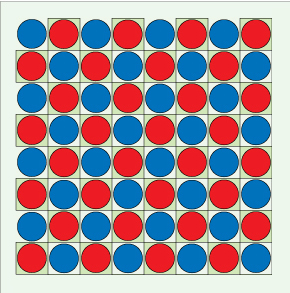
\includegraphics[scale=0.8]{resources/initial-state.jpg}
    \caption{Estado inicial do jogo}
    \label{fig:initial-state.png}
\end{figure}

\subsection{Visualização do Tabuleiro}

O tabuleiro pode ser visualizado pela linha de comandos a cada nova jogada efetuada quer pelo utilizador quer pelo computador.
É disponibilizada informação acerca das peças ainda em jogo, e auxiliares na seleção de jogadas como a letra representativa de uma coluna e um número para uma linha.

\begin{figure}[H]
    \center
    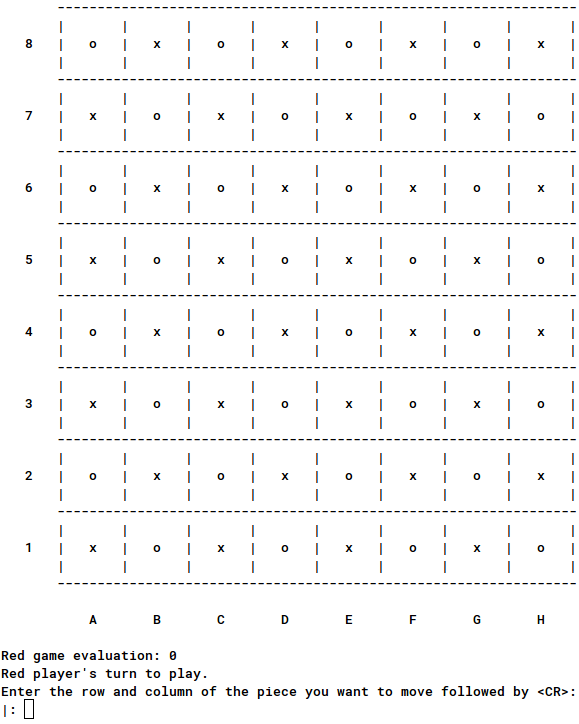
\includegraphics[scale=0.5]{resources/piece-selection.png}
    \caption{Estado inicial do jogo com pedido de seleção de jogada}
    \label{fig:piece-selection.png}
\end{figure}

\subsection{Lista de Jogadas Válidas}
Não está implementado nenhum método que angarie um conjunto de jogadas válidas, no entanto é possível determinar se existem movimentos válidos para uma dada peça do tabuleiro, sem movimentar nenhuma peça do tabuleiro, através de uma chamada à função \texttt{check\_move\_availability}.

\begin{lstlisting}[style=customprolog]
check_move_availability(SrcRow, SrcCol, Player, Board):-
	% a move must be checked in all directions
	IncRow is SrcRow + 1,
	DecRow is SrcRow - 1,
	IncCol is SrcCol + 1,
	DecCol is SrcCol - 1,
	(
	   IncRow =< 7, validate_move(SrcRow, SrcCol, IncRow, SrcCol, Player, Board, _, _);
	   DecRow >= 0, validate_move(SrcRow, SrcCol, DecRow, SrcCol, Player, Board, _, _);
	   IncCol =< 7, validate_move(SrcRow, SrcCol, SrcRow, IncCol, Player, Board, _, _);
	   DecCol >= 0, validate_move(SrcRow, SrcCol, SrcRow, DecCol, Player, Board, _, _);
	   DecRow >= 0, DecCol >= 0, validate_move(SrcRow, SrcCol, DecRow, DecCol, Player, Board, _, _);
	   IncRow =< 7, IncCol =< 7, validate_move(SrcRow, SrcCol, IncRow, IncCol, Player, Board, _, _);
	   DecRow >= 0, IncCol =< 7, validate_move(SrcRow, SrcCol, DecRow, IncCol, Player, Board, _, _);
	   IncRow =< 7, DecCol >= 0, validate_move(SrcRow, SrcCol, IncRow, DecCol, Player, Board, _, _)
	), !.
\end{lstlisting}

\subsection{Execução de Jogadas}
No caso da seleção de uma jogada manualmente através da consola, com a introdução de uma letra a representar a coluna e um número a representar uma linha, o programa tenta validar e mover uma peça do tabuleiro, tentando primeiro fazer uma jogada do tipo de salto. Quando o salto falha, são tentados outros dois tipos de movimentos: um adjacente e por fim, em último recurso, um movimento centralizador. Caso nenhum movimento seja válido, de acordo com as regras, assume-se que o jogador tem de dar a vez ao seu adversário. Em nenhum caso o jogo pode ficar numa situação na qual nenhum dos dois jogadores está sem jogadas válidas para executar.

\begin{lstlisting}[style=customprolog]
make_move(SrcRow,SrcCol, DestRow, DestCol, Game, ModifiedGame):-
	(       
	   nl, write('Attempting to make a jump move...'), nl,
	   make_jump(SrcRow,SrcCol, DestRow, DestCol, Game, TemporaryGame);
	
	   write('Failed to make a jump move!'), nl, nl,
	   write('Attempting to make an adjoining move...'), nl,
	   make_adjoining_move(SrcRow,SrcCol, DestRow, DestCol, Game, TemporaryGame);
	
	   write('Failed to make an adjoining move!'), nl, nl,
	   write('Attempting to make a centering move...'), nl,
	   make_centering_move(SrcRow,SrcCol, DestRow, DestCol, Game, TemporaryGame);
	
	   write('Failed to make a centering move!'), nl, nl,
	   get_board(Game, Board), get_player_turn(Game, Player),
	   check_move_availability(SrcRow, SrcCol, Player, Board), ModifiedGame = Game;
	
	   write('No valid moves were available -> Switching player turn!'), nl, nl,
	   change_player_turn(Game,ModifiedGame), true
	),
get_force_jump(TemporaryGame, ForceJumpMode),
(
   ForceJumpMode == noForceJump -> change_player_turn(TemporaryGame,ModifiedGame),! ;
   ModifiedGame = TemporaryGame
).
\end{lstlisting}

\subsection{Avaliação do Tabuleiro}
Apesar de ser feita uma avaliação simples do estado do jogo, não é feito nenhum aproveitamento para além da visualização deste valor no início de cada jogada. É feito um cálculo da avaliação do tabuleiro para um dado jogador, com a diferemça do seu número de peças com o número de peças do adversário. Neste jogo em específico, é um cálculo relativamente acertado, ignorando os casos em que, no turno em vigor é possível fazer múltiplos saltos, sendo a avaliação um valor subestimado.

\begin{lstlisting}[style=customprolog]
get_evaluation(Game,Player,Evaluation):-
    get_num_red_pieces(Game, NumRedPieces),
    get_num_blue_pieces(Game, NumBluePieces),
    (
       Player == redPlayer -> Evaluation is NumRedPieces - NumBluePieces;
       Player == bluePlayer -> Evaluation is NumBluePieces - NumRedPieces
    ),!.
\end{lstlisting} 

\subsection{Final do Jogo}
Em cada iteração do ciclo principal do jogo, é feita a verificação do número de peças no tabuleiro. Quando um ou mais jogadores tiver zero peças em cima do tabuleiro o jogo está terminado e o vencedor foi o último jogador que fez uma movimentação no tabuleiro. É de salientar a possibilidade de o tabuleiro final estar completamente vazio, sendo o vencedor aquele que fez o salto final e que eliminou uma peça inimiga para fora do tabuleiro.

\begin{lstlisting}[style=customprolog]
validate_board_pieces(Game):-
    get_num_red_pieces(Game,NumRedPieces),
    get_num_blue_pieces(Game,NumBluePieces),
    NumRedPieces > 0,
    NumBluePieces > 0,!.
\end{lstlisting}

\begin{figure}[H]
    \center
    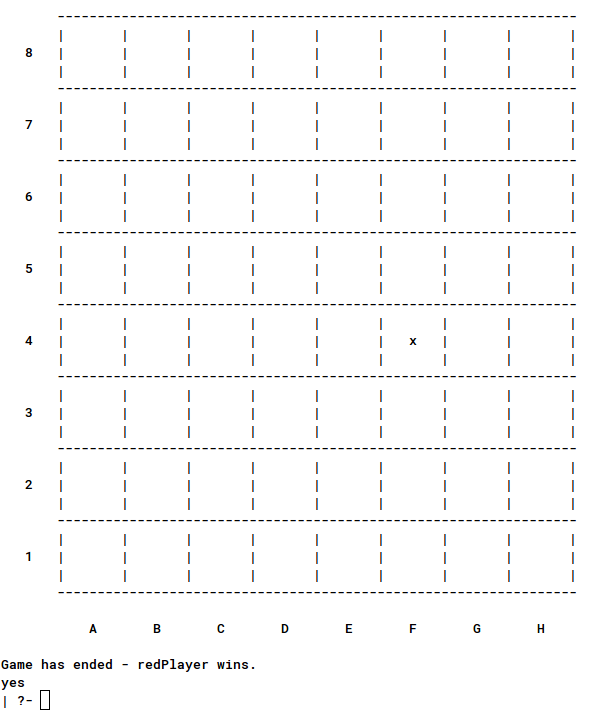
\includegraphics[scale=0.5]{resources/game-ending.png}
    \caption{Estado final de um jogo com declaração de vencedor}
    \label{fig:game-ending.png}
\end{figure}

\subsection{Jogada do Computador}
Não está implementada a possibilidade de seleção do modo de dificuldade de uma jogada do computador. O computador executa jogadas de forma aleatória.


%%%%%%%%%%%%%%%%%%%%%%%%%%
\section{Interface com o Utilizador}

No primeiro contato que o utilizador tem com o programa é-lhe solicitado o modo de jogo que permite, estando à disposição três distintos: humano contra humano, humano contra computador e computador contra computador.

\begin{figure}[H]
    \center
    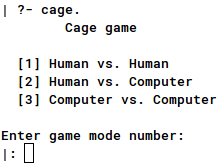
\includegraphics[scale=0.6]{resources/main-menu.png}
    \caption{Menu inicial do jogo}
    \label{fig:main-menu.png}
\end{figure}

A partir do momento em que o utilizador escolhe o modo de jogo computador contra computador, o programa inicia e finaliza rapidamente um jogo cujos movimentos são escolhidos pela simulação e execução aleatória de jogadas de forma automática. Nos outros dois modos de jogo, é pedida a introdução de uma jogada. 


%%%%%%%%%%%%%%%%%%%%%%%%%%
\section{Conclusões}
Após a realizão deste projeto, concluí-mos que ainda temos muito pouco à vontade no desenvolvimento de procedimentos de programação em lógica e que muitos dos hábitos herdados de programação de outras linguagens nos trouxeram muitas situações ante problemas dos quais ainda não sabemos como contornar. É também de criticar a complexidade exagerada do trabalho, considerando o nosso conhecimento limitado e inexperiência na linguagem em questão, sendo que propunhamos este nível de complexidade apenas a partir de um segundo trabalho, ou um prazo de entrega mais alargado para este primeiro projeto.

\begin{thebibliography}{9}
\bibitem{lamport93}
  Sterling, Leon
  \emph{The Art of Prolog},
  The MIT Press
  2nd edition,
  2000.
  
  \bibitem{bl}Abstract games,
  \url{http://www.marksteeregames.com/MSG_abstract_games.html}, 14 10 2016.
  
  \bibitem{bl}Cage rules,
  \url{http://www.marksteeregames.com/Cage_rules.html}, 14 10 2016.
\end{thebibliography}

\newpage
\appendix
\section{Código fonte}
Código Prolog implementado devidamente comentado e outros elementos úteis que não sejam essenciais ao relatório.

\end{document}
